\chapter{系统设计}
\label{chp:design}





\todo{
为了了解Android 应用程序在运行阶段的执行过程,本文提出了一个可用于还原Android应用程序运行时动态函数调用图的工具——RunDroid。
}
RunDroid利用源程序代码插桩和运行时方法拦截的相结合的方式,捕获应用程序在应用层面和系统层面的方法执行信息,还原方法间的调用关系。
在此基础上,RunDroid利用对象和方法的关系结合具体的触发规则,进而还原出方法间触发关系,在调用图中展现运行过程中的Android特性行为。
RunDroid提供的函数调用图从方法调用关系、方法间的触发关系以及方法执行的相关对象信息等多个方面较为全面地刻画了Android应用程序的执行过程。


\section{整体设计}



\begin{figure*}[!ht]
	\centering
	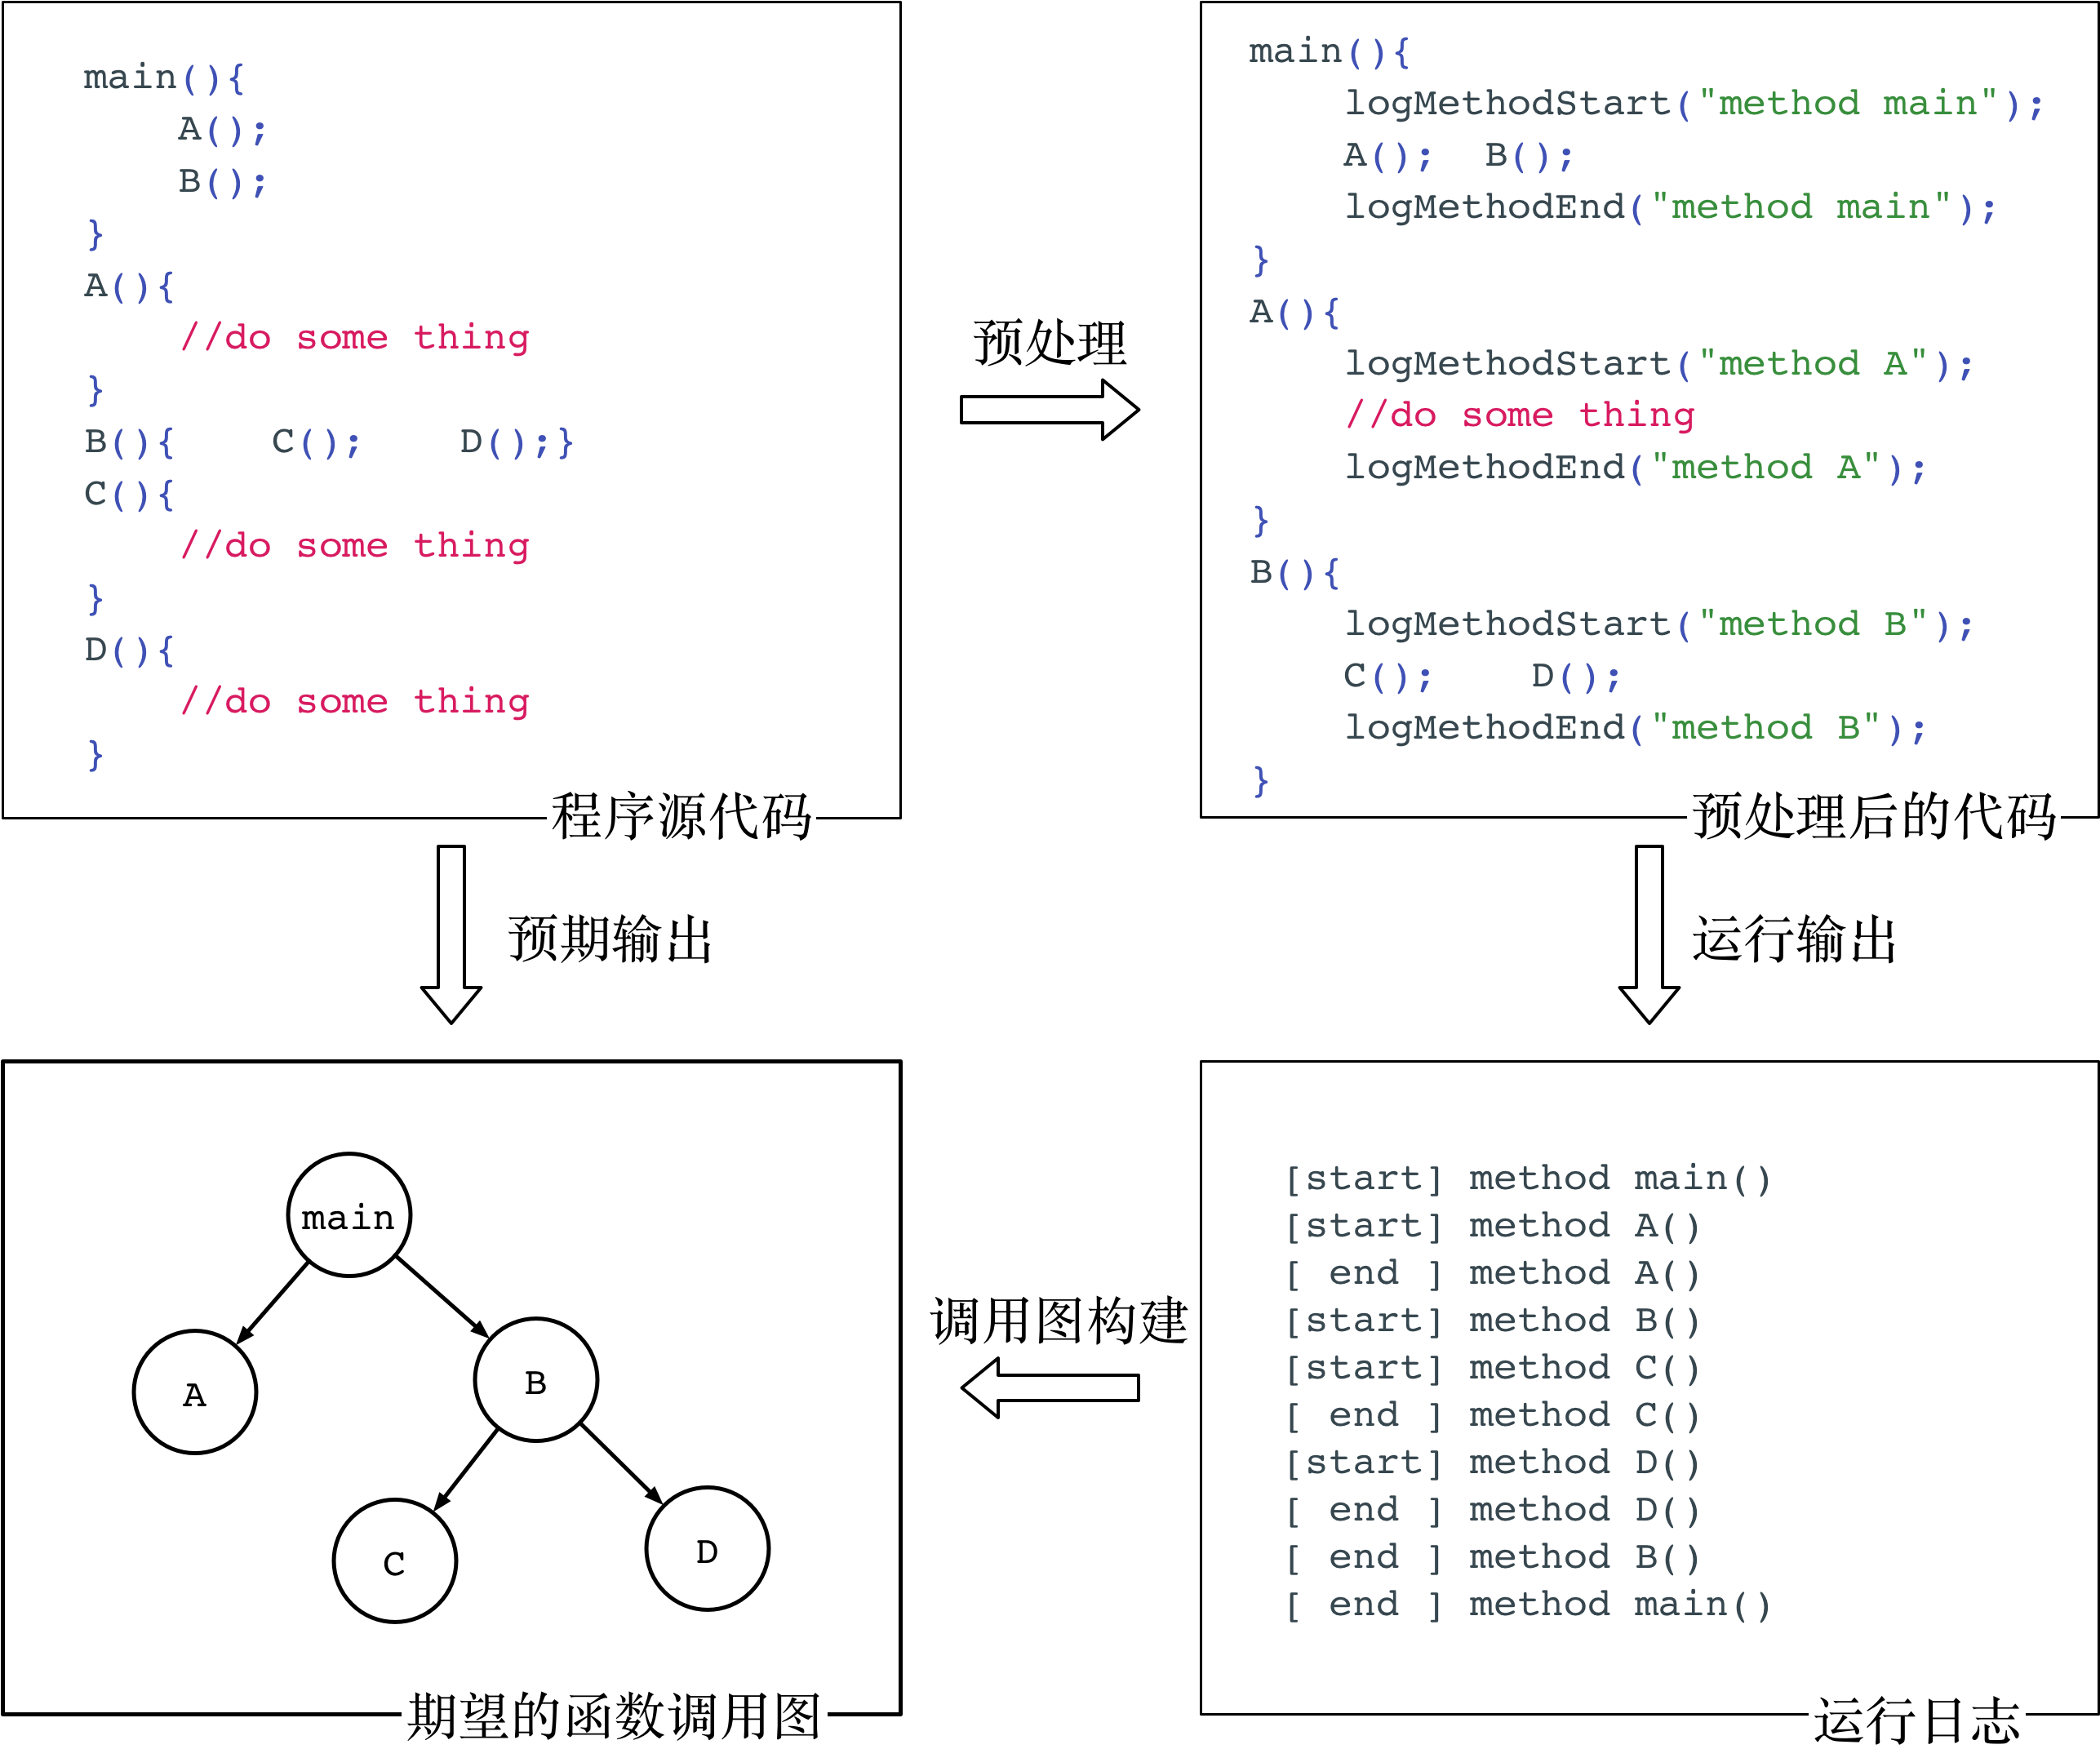
\includegraphics[width=0.8\textwidth]{./Figures/code-sample.png}
	\caption{RunDroid的处理流程}
	\label{fig:code_sample}
\end{figure*}


%在本节,
%以\autoref{fig:code_sample}为例,%简要介绍一下RunDroid还原Android应用程序的函数调用图的基本思路:
\autoref{fig:code_sample}-左上为一段示例代码:在main函数执行时,程序会依次调用A、B两个函数,而B函数则会调用了C、D两个函数。
\autoref{fig:code_sample}-左下则是程序的运行时函数调用图,即RunDroid实际的输出产物。
程序执行过程可以看做函数调用图的深度优先遍历过程。
还原函数调用图的关键点,在于如何在程序执行过程中输出树的遍历序列,并根据遍历序列进行还原函数调用图。
\eat{
通常的,树的遍历分为中序遍历、前序遍历以及后序遍历三种。
但是,两颗结构完全不同的树对应的遍历序列可能是一样的,
这也就意味着上述三种遍历方法均不能直接还原出函数调用图。
而且,函数执行过程中出现的错误异常可能使得序列输出中断,阻碍调用图的构建。
}
%本文采用的方案是利用在方法执行前后均记录执行日志(即一个方法的执行会输出两条日志:方法开始日志、方法结束日志),
%进行动态函数调用图的还原。

本文采用的方案:
RunDroid通过对源程序(\autoref{fig:code_sample}-左上)进行预处理,得到包含日志记录功能的运行代码(\autoref{fig:code_sample}-右上);
程序在函数执行前后可以输出和方法执行相关的日志信息,(\autoref{fig:code_sample}-右下);
最后,我们根据这些日志信息构建出函数调用图(\autoref{fig:code_sample}-左下)。
另外,在函数调用图的基础上,RunDroid利用日志中包括的方法对象信息,挖掘和方法对象相关联的方法,结合具体触发规则,进而建立方法触发关系。

% 从函数调用图的构建过程可以看出,程序的执行过程就是对函数调用图自上而下的深度优先遍历过程。由此可见,若要还原出图 6-右中的函数调用图,本文采用的基本思路是以日志方式输出对右图中的函数调用图的深度优先遍历序列,并基于得到的遍历序列还原出函数调用图。
% 由于Android是由面向对象编程语言Java开发的系统,系统还需要考虑面向对象编程的特性——多态性(即同一个行为在不同的对象下的表现可以不同)。为此,RunDroid还会在函数调用图将函数执行和对应的对象进行关联,更好地体现面向对象编程的函数调用关系。基于上述的函数调用关系的信息,RunDroid根据函数调用之间的关系进一步挖掘,进一步挖掘Android系统中的特性(例如组件Activity的生命周期、多线程的交互方式)。
%\section{总体框架}
\eat{


\begin{figure*}[!ht]
	\centering
	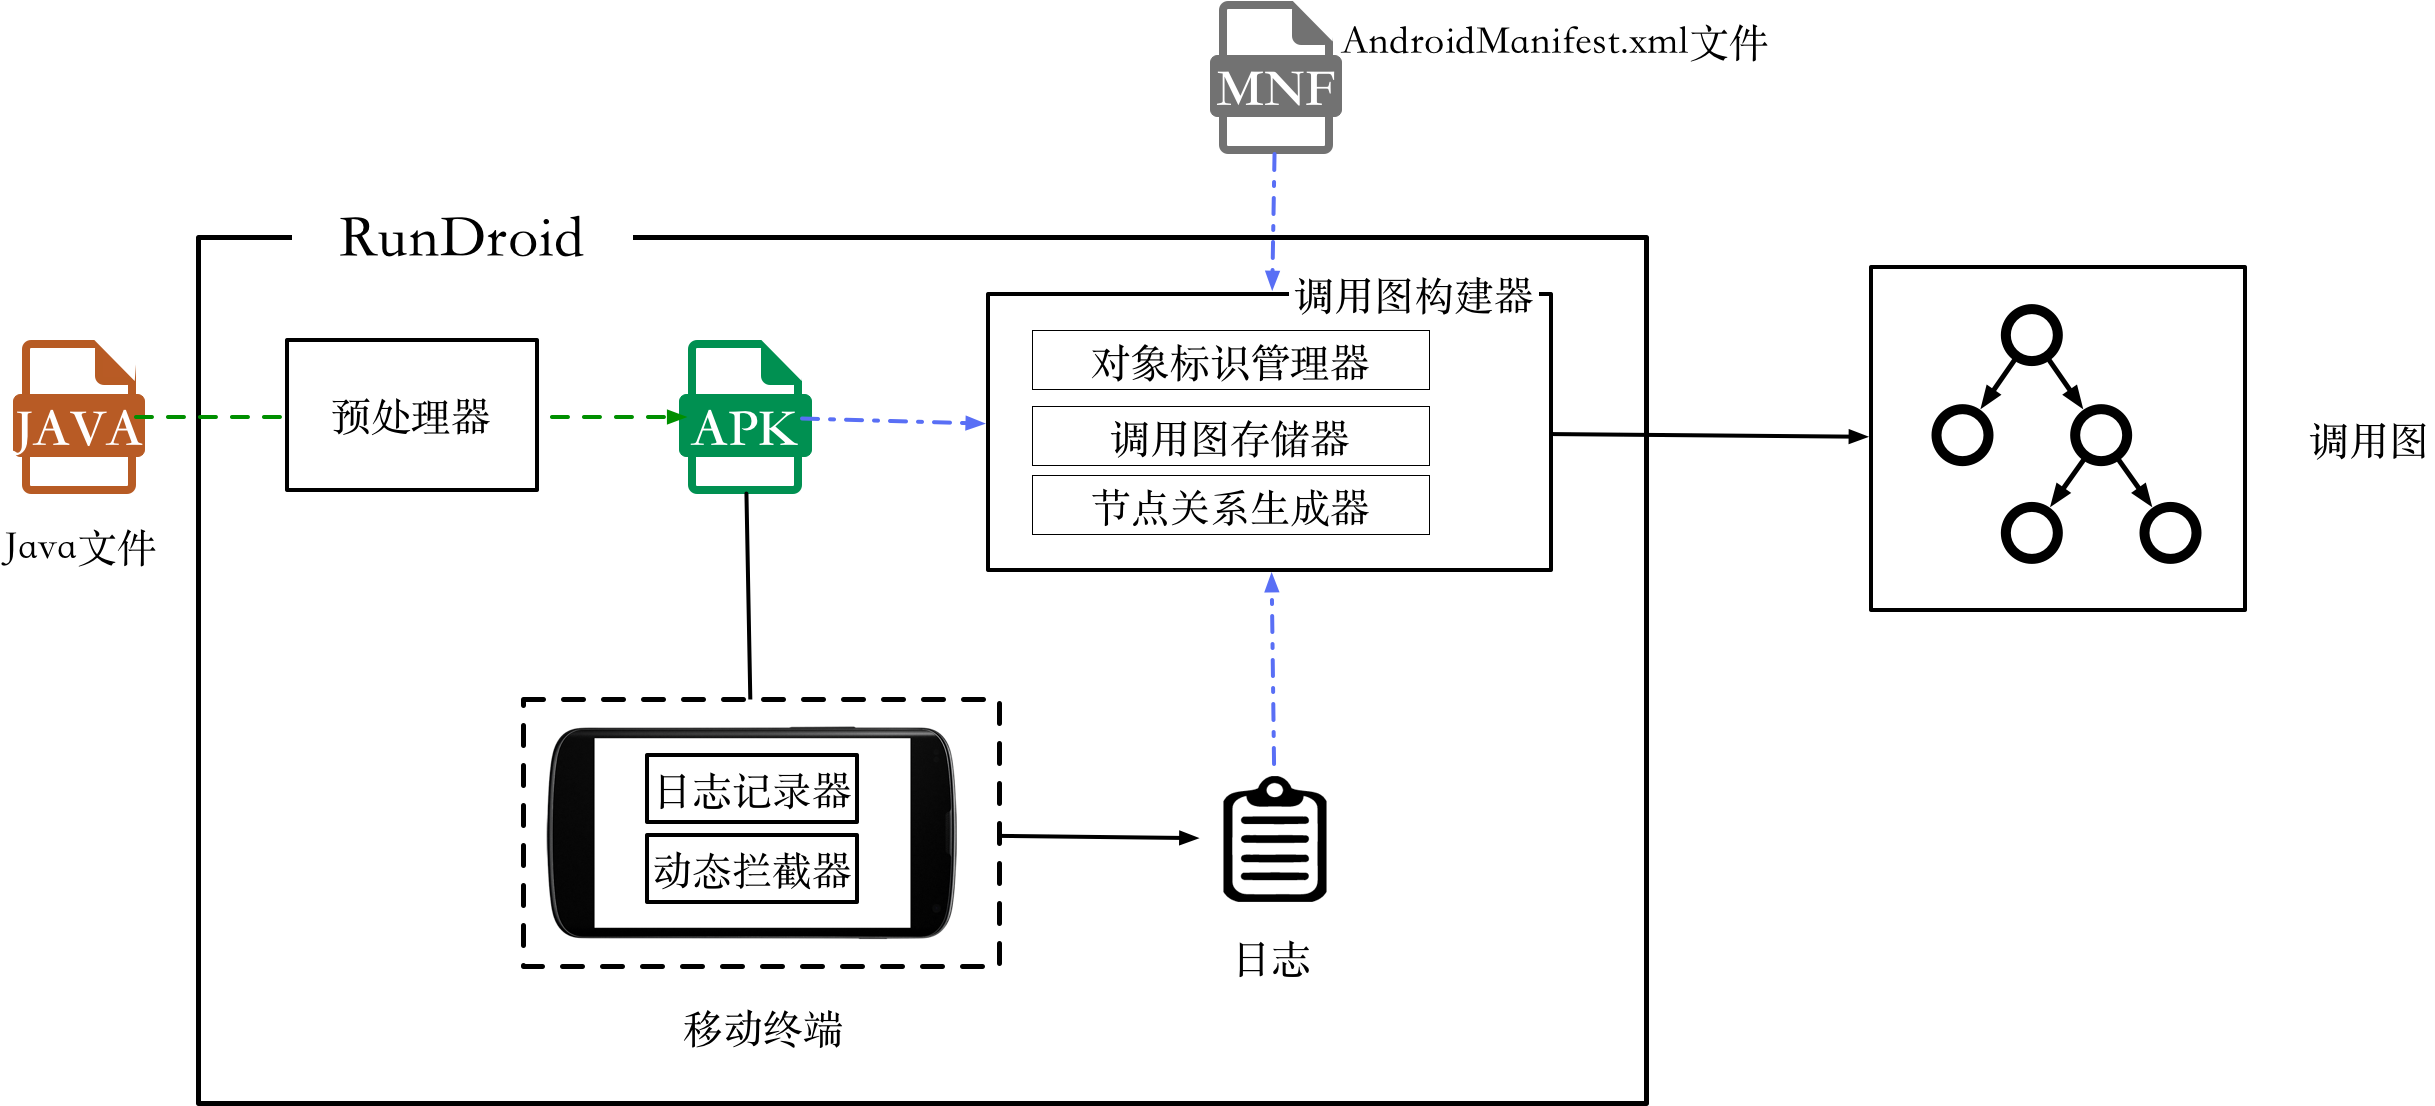
\includegraphics[width=0.8\textwidth]{./Figures/rundroid-overview.png}
	\caption{ RunDroid的工作流程}
%	\label{fig:rundroid_overview}
\end{figure*}

在技术实现上,RunDroid主要分为预处理器、运行时拦截器、日志记录器、调用图构建器等4个部分,对应的工作流程如\autoref{fig:rundroid_overview}所示。
从功能上,预处理器和运行时拦截器两者的作用是一致的:在程序运行过程中,当相关方法执行时,触发日志记录器记录相应的信息。
预处理器通过源代码插桩技术实现在用户方法运行时触发用户方法的信息记录,而运行时拦截器则是通过方法劫持技术实现对系统方法执行的拦截,进而触发日志记录。
%系统方法的执行。
%由于,用户方法层面的代码已修改,而系统方法的行为难以修改
%并非所有的方法都是进行日志代码织入的。RunDroid可以接触到用户方法(开发者在应用层面定义的方法)的源代码,而对于前者,
在应用运行时,日志记录器会以日志的形式将用户方法和系统方法对应的执行信息记录下来。
最后,调用图构建器会根据应用程序运行时输出的日志,构建拓展函数调用图。
}


%接下来,本章将从方法信息捕获和拓展调用图构建两个方面介绍RunDroid的设计。


% 本技术路线拟利用语法分析工具,对Android应用程序进行了应用源代码层面的执行日志插桩工作,利用非侵入式系统行为修改插件获取系统层面的函数执行信息。
% 结合以上日志信息,方案对日志进行初步处理,在图数据库上构建原始的Android应用程序的动态函数调用图。
% 通过阅读分析Android系统中多线程相关的源代码,制定具体的多线程分析插件,进而在函数调用图中标识出多线程相关的方法间触发关系,
%全面地展现Android应用的执行过程。


\section{方法信息的捕获}

\todo{在RunDroid中,方法一共分为两类,用户方法和系统方法。}
用户方法是由用户定义的,直接修改的成本较低,易于实现。
而系统方法在系统中定义,属于系统运行环境的一部份,行为修改成本较高。
虽然记录这两种方法的执行信息的方式是不一样的。
但是两者最终的效果是一致的:当应用程序运行时,相关方法的执行信息均会\todo{通过日志记录器记录下来},用于后续调用图的构建。


\subsection{用户方法执行信息的获取}%——基于源代码的日志代码插桩过程}


\todo{预处理器以Android项目源代码作为输入,输出预处理后的APK文件。}
%输出的APK文件在应用执行过程中将用户方法的执行信息输出出来。
具体处理过程如\autoref{alg:instrument}所示:
\todo{预处理器会}遍历项目源代码中的Java源文件,将源文件和对应的抽象语法树转化成XML格式的文件,并以DOM的形式加载到程序中(第3行)。
%  利用获取的语法结构,预处理器会提取出所有的方法体,
对于抽象语法树中的每一个类和每一个方法,预处理器会计算出编译后所处的类的全限类名及方法签名(第4$\sim$\ref{alg:instrument:computeMethodId}行)。
全限类名和方法签名的组合<全限类名,方法签名>可以作为方法体的唯一标识,和抽象语法树中的方法体一一对应。
在每个方法内部,预处理器会插入用户方法日志记录的代码,实现日志代码编织,达到用户方法运行时信息记录的目的(第\ref{alg:instrument:addMethodExitLogCode}$\sim$\ref{alg:instrument:addMethodEnterLogCode}行)。
另外,预处理器还对每个方法体进行了异常捕获处理,防止方法体内部的异常导日志记录过程的中断,影响函数调用图的构建(第\ref{alg:instrument:addMethodCatchLogCode}行)。
上述操作都是对DOM对象\code{document}直接操作的。
当一个Java文件修改完毕后,预处理器会将DOM对象重新转换成Java源文件,并替换原来的文件(第\ref{alg:instrument:rewriteFile}行)。
最后,预处理器会利用编织后得到的源代码构建成APK文件(第\ref{alg:instrument:buildApk}行)。




\begin{algorithm}[!ht]
	\caption{日志代码插桩过程} 
	\label{alg:instrument}
	\KwIn{ $javaFiles$,应用程序的源代码}
	\KwOut{ $apk$,包含插桩代码的APK文件}
	\SetKwProg{Fn}{Function}{:}{}
	
	\Fn{buildApk($log$)}{
		
		\For{$ javaFile \in javaFiles $}{
			

			将源文件 $javaFile $ 的抽象语法树转化成DOM对象 document;
						
			\For{ \emph { $ classEle \in document$}}{
				
				$className $ ~ $\gets  $ ~ computeClassName($classEle$,$xmlFile$); 	
				
				\For{\emph { $methodEle \in  classEle $}}{
					
					$methodId $ ~ $\gets $~ computeMethodId($methodEle$,$className$ ); 	 \label{alg:instrument:computeMethodId}
					
					addMethodExitLogCode($methodEle$,$methodId$);\label{alg:instrument:addMethodExitLogCode}
					
					addMethodCatchLogCode($methodEle$,$methodId$);  \label{alg:instrument:addMethodCatchLogCode}
					
					addMethodEnterLogCode($methodEle$,$methodId$);\label{alg:instrument:addMethodEnterLogCode}
				}
				
			}
		将  $document$ 转化成新的Java文件 $newJavaFile$; \label{alg:instrument:rewriteFile}
			
		}
		$	apk  \gets$ buildApk($newJavaFiles$)  \label{alg:instrument:buildApk}
		
		\KwRet{apk };
	}
	
\end{algorithm}
\subsection{系统方法执行信息的获取}%——基于动态拦截技术的方法信息捕获}



运行时拦截器的主要职责是对Android系统方法的执行进行拦截,将相关信息传递给日志记录器并记录下来。
运行时拦截器维护着系统方法列表。
列表中的方法通常和Android特性相关,例如Activity的生命周期方法、Java Thread API以及Handler相关的API,具体如\autoref{tbl:hookMethodList}所示。
在目标应用程序开始运行前,运行时拦截器会为上述目标方法注册执行回调函数。
在目标方法执行前和执行后,对应的回调函数会被执行,进而通过日志记录器记录下这些方法执行的相关信息。
在RunDroid中,运行时拦截器可以弥补预处理器无法提供系统方法执行信息的不足,填补调用图缺失的系统方法执行,进而还原出应用层和系统层之间以及系统内部的方法调用,使得产生的调用图更加完整。

{
\begin{table*}[!ht]
	%	\centering
	\footnotesize		
	
	\caption{运行时拦截器拦截的系统方法列表}
	
	\label{tbl:hookMethodList}
	
	
	\resizebox{\textwidth}{!}{
		\begin{threeparttable}[b]
			
			\begin{tabular}{|l|c|}
				\hline
				方法签名&说明\\
				\hline
				Activity.onCreate(Bundle)   &\multirow{6}{0.4\linewidth}{和Activity生命周期相关的方法}\\
				%	\cline{1-1}
				Activit.onStart()    &\\
				Activity.onResume()     &\\
				Activity.onPause()    &\\	
				Activity.onStop()     &\\
				Activity.onDestroy()    &\\
				\hline
				
				Thread.start()   & 和Java 线程启动相关的方法\\
				\hline
				Message.obtain() & \multirow{15}{0.4\linewidth}{和 Hanlder机制相关的方法}\\
				Handler.enqueueMessage(MessageQueue,Message,long)&\\
				Handler.dispatchMessage(Message)&\\
				Handler.post(Runnable)&\\
				Handler.postAtTime(Runnable,long)&\\
				Handler.postAtTime(Runnable,Object,long)&\\
				Handler.postDelayed(Runnable,long)&\\
				Handler.postAtFrontOfQueue(Runnable)&\\
				Handler.sendMessage(Message)&\\
				Handler.sendEmptyMessage(int)&\\
				Handler.sendEmptyMessageDelayed(int,long)&\\
				Handler.sendEmptyMessageAtTime(int,long)&\\
				Handler.sendMessageAtFrontOfQueue(Message)&\\
				Handler.sendMessageDelayed(Message,long)&\\
				Handler.sendMessageAtTime(Message,long)&\\
				
				\hline
				
				
				%		AsyncTask execute [Object& \multirow{3}{0.4\linewidth}{和 AsyncTask相关的方法}\\
				%		AsyncTask publishProgress [Object&\\
				%		AsyncTask executeOnExecutor Executor [Object &\\
				%		\hline
				
				
			\end{tabular}
			
			%		\begin{tablenote}
			%		\end{tablenote}
			
		\end{threeparttable}
	}
\end{table*}
}
\section{扩展函数调用图的构建过程}

调用图构建器构建拓展函数调用图的过程分为如下几个阶段:
 RunDroid根据程序运行时的日志提取函数间的调用关系,创建函数调用图;
根据AndroidManifest.xml的Activity组件声明,在函数调用图上标识出完整的Activity 生命周期流转序列;
利用方法执行与方法对象的关联关系,结合触发关系规则,补全方法间的触发关系,形成最终的拓展函数调用图。




\begin{algorithm}[ht]
	\caption{函数调用图的构建过程} 
	\label{alg:buildCG}
	\KwIn{ $logs$,应用程序的运行时日志}
	\KwOut{ $ecg$, 拓展函数调用图}
	\SetKwProg{Fn}{Function}{:}{}
	
	\Fn{buildExtendedCallGraph($log$)}{
		
		$ecg$ $\gets$ new ExtendedCallGraph();
		
		\For{thread $\in$ $logs.threads$}{
			
			$stack$ $\gets$ new Stack();
			
			\For  {$log$ $\in$ $logs.get(thread)$}{
				
				$top$ = $stack$.peek() ;  
				
				\eIf{isMethodStartLog($log$)} {
					
					$m \gets $ generateMethodInfo($log$);
					
					$ecg$.addMethodNode($m$);
					%\Comment 在调用图中提交方法节点 
					
					$ecg$.addMethodObjectsIfNotExists($ o_p $,$o_i $) 	;							
					
					$ecg$.addMethodObjectRels($ \left\langle  o_p \joinrel\xrightarrow{parameter}   m \right\rangle   $,$ \left\langle  o_i \joinrel\xrightarrow{instance}   m \right\rangle  $) ;
					
					%	\Comment 在调用图中提交方法对象节点 (此处只涉及参数关系和实例关系)
					
					\If {  $top \neq null $ }{
						
						$ecg$.addInvokeRel($ \left\langle  top \to  m \right\rangle  $) ;
						
						$stack$.push($m$);
					}
					
				}{ 
					
					$ecg$.addMethodObjectIfNotExists($  o_r  $) ;
					
					$ecg$.addMethodObjectRel($ \left\langle   o_r \joinrel\xrightarrow{return}   m \right\rangle  $) ;
					
					%		  \Comment 在调用图中提交方法对象节点 (此处只涉及返回值关系)
					
					$stack$.pop() ;
					
				}
				
				
				
			}
		}
		\KwRet{ $ecg$};
	}
	
\end{algorithm}
\subsection{构建函数调用图}

%虽然所有线程的方法日志输入到同一个文件中,但是,从单个线程的视角看这些日志,日志在时间维度上的先后顺序就是对调用图的深度遍历。
%已检测的应用程序将日志输出到单个文件中。
%虽然所有线程的日志都输出到一个日志文件中,但在每个线程的视图中,日志条目的输出顺序遵循调用图的顺序遍历:调用方法在被调用方法之前输出。
%此外,每个方法执行对应于两个日志条目:方法入口和出口的日志条目。

由于\todo{各个线程}在执行过程中,不存在一个调用关系跨越两个线程,因此,在整个构建过程中,RunDroid以产生日志的线程为基本构建单元,向调用图添加方法调用关系。
函数调用图的构建过程如\autoref{alg:buildCG}所示。

对于每个线程,RunDroid顺序遍历对应的日志,使用栈$stack$的入栈、出栈操作来模拟对应线程的函数执行的过程,还原调用关系(第2$\sim$ 20行):
当读取到方法执行的开始日志时,系统会在调用图创建一个节点表示该方法的执行(第7$\sim$8行),
同时也在调用图中添加方法参数、方法实例对应的对象节点$o_p$、$o_i$以及方法对象和方法的关系$ \left\langle  o_p \joinrel\xrightarrow{parameter}   m \right\rangle   $、$ \left\langle   o_i \joinrel\xrightarrow{instance}   m \right\rangle  $(第9$\sim$10行)。
如果此时当前线程栈$stack$的栈顶方法元素$top$存在,系统会创建从方法$top$到当前方法$m$的调用关系,$\left\langle top \to m \right \rangle  $,并将当前方法$m$压入栈$stack$中(第11$\sim$ 14行)。
当读取到方法执行的结束日志时,该日志对应的方法必然是栈顶方法$top$,若栈顶方法$top$存在返回对象$o_r$,则只需要将$o_r$和$top$的关系添加到调用图中即可,最后弹出栈顶的$top$即可(第 16$\sim$ 18行)。
在上述过程中,如果待添加的方法对象在调用图中已经存在时,该对象复用调用图原有的对象节点即可,无须重新添加,只需添加方法与对象间的关系即可。




% 当日志条目表示方法条目时,将根据日志条目和来自的4元组信息创建节点 日志存储在节点中(第6行)。
%然后,从堆栈顶部的方法到日志条目中的方法(第7-9行)构建调用关系。
%处理完调用关系后,该方法将被推入堆栈。当日志条目表示方法退出时,堆栈将弹出顶部的方法节点(第11-12行)。
%重复该过程,直到没有为一个线程留下日志条目,然后将为日志文件中的另一个线程启动相同的进程。

%构建扩展调用图。 
%DROIDSTITCHER通过添加表示已识别触发关系的边来扩展调用图。
%请注意,触发器关系中的目标方法通常是回调方法的调用图的入口点。
%因此,通过将触发关系添加为边,将所有调用图拼接成一个调用图作为输出。



\subsection{构建Activity的生命周期和事件回调}

\point{构建Activity的生命周期}


\begin{algorithm}[!hb]
	\caption{构建Activity的生命周期和事件回调} 
	\label{alg:buildActivityLifecycle}
	\KwIn{ $manifestFile$,AndroidManifest文件\\ \qquad  \quad $ecg$,函数调用图}	
	\KwOut{ $ecg$,包括Activity生命周期的函数调用图}
	
	
	
	\SetKwProg{Fn}{Function}{:}{}
	
		\Fn{patchActivityLifecycleAndUiEvent($ecg$)}{
		
		patchActivityLifecycle($ecg$,$manifestFile$);
		
		patchUiEvent($ecg$);

		\KwRet{$ecg$};
	}
	
	
	\Fn{patchActivityLifecycle($ecg$,$manifestFile$)}{
		
		
		$lifecycleList \gets$ new   $ List()$;
		
		
		\For{ \emph{ $o_{activity} \in \{ act \mid act $ 为文件 $manifestFile $中定义的Activity$ \} $ }}{
			
			
			
			\For{ \emph{ $m \in \{ m \mid  m$ 为调用图 $ ecg $中以$o_{activity}$为实例的方法节点$\}$}}{
				
				
				\If{ \emph{ $m$ 为Activity的生命周期方法  \\\qquad
						\&\&   $m$ 的执行线程为主线程\\\qquad
						\&\&  $  \left\langle  m' \to m \right\rangle  \notin ecg$
				} }{
					
					$lifecycleList$.add($m$);
				}
				
				
			}
		}
		
		sortListByTime($lifecycleList$);
		
		linkItemsByTime($lifecycleList$,$ecg$);
		
	}
	% $o_p \stackrel{parameter}{\longrightarrow} m$
	\Fn{patchUiEvent($ecg$)} {
		\For{\emph{$o_{view} \in \{ o \mid o $ 为调用图 $ ecg $中\code{View}类型的对象节点  $ \}$} }{ 
			\For{\emph{$o_{listener} \in \{ o \mid o $  为调用图 $ ecg $  中\code{View.OnClickListener} 类型的对象节点 $ \}$} }{		
				\If {\emph{$o_{view}$,$o_{listener}$,$m_{register}$ 和 $m_{click}$  满足\autoref{equ:rule_ui}}
					}{
					$ecg$.addTriggerRel($m_{register} \lhook\joinrel\xrightarrow{UiEvent}  m_{click} $)	
				}
			}
		}
	}		
\end{algorithm}


	
Android 应用的Acticvity生命周期的构建就是将Activity生命周期方法按照时间顺序串联起来。%,利用的是\code{Activity}生命周期方法的签名的不变性。
生命周期的构建过程以AndroidManifest文件作为输入,在原有的函数调用图的基础上,添加\todo{表示Activity生命周期}的有向边,具体过程如\autoref{alg:buildActivityLifecycle}所示:
对于AndroidManifest文件中声明的每一个Activity组件对象 $o_{activity}$,系统都会遍历以该对象为方法实例的方法$m$(即$m$、$o_{activity}$满足条件$o_{activity} \joinrel\xrightarrow{instance} m$);
若方法$m$同时满足三个条件,则将它添加到列表$lifecycleList$中(第7$\sim$12行)。
最后,将列表$lifecycleList$按照时间顺序进行排序,并依次连接起来,即可得到\code{Activity}的生命周期(第13$\sim$14行)。

这三个条件分别为:
(1)方法$m$的方法签名和\autoref{fig:Activity-lifecycle}中的任何一个生命周期方法的签名保持一致;
(2)方法$m$执行时所处的线程为主线程;
(3)\todo{
方法$m$在调用图$cg$中不在调用者,即在调用图$cg$中不存在方法$m' \in cg$,使得$m' \to m $成立。
}

\point{构建Andoid事件回调的触发关系}

在构建Andoid事件回调的触发关系时,我们会遍历拓展调用图中的所有\code{View}类型的对象节点$o_{view}$和\code{View.OnClickListener}类型的对象节点$o_{listener}$的组合。
对于组合$\left\langle o_{listener}  , o_{view}\right\rangle $,若调用图中存在方法节点$m_{register} $、$m_{click} $满足\autoref{equ:rule_ui},方法节点$m_{register} $、$m_{click} $之间添加从$m_{register} $指向$m_{click} $的有向边,即$m_{register} \lhook\joinrel\xrightarrow{UiEvent}  m_{click}  $(第16$\sim$19行)。


%Andoid事件回调的触发关系描述的是控件点击事件的注册和响应之间的因果关系,即方法\code{View.setOnClickeListener(View\$OnClickListener)}(用$m_{register}$表示)和\code{View\$OnClickListener.onClick(View)}间的因果关系(用$m_{click}$表示)。
%根据第\ref{chp:definition}章中方法触发关系的相关定义,$m_{register} \lhook\joinrel\xrightarrow{UiEvent}  m_{click}  $ 成立。
%我们观察发现:方法$m_{register}$的实例对象$o_{view}$是方法$m_{click}$的参数对象,而方法$m_{register}$的参数对象$o_{listener}$是方法$m_{click}$的实例对象。
%因此,在构建Andoid事件回调的触发关系过程中,当方法$m_{register} $、$m_{click} $满足第19$\sim$22行的条件时,这两个方法之间存在触发关系,即$m_{register} \lhook\joinrel\xrightarrow{UiEvent}  m_{click}  $(第23行)。


\eat{
基于Java的多线程交互往往是以\code{Runnable}作为传递对象,通常通过调用方法\code{Thread.start()} (用$m_{start}$表示)和\code{Activity.runOnUiThread(Runnable)}(用$m_{runOnUiThread}$表示)等API,进而触发方法\code{Runnable.run()}(用$m_{run}$表示)的执行。
因此,对于方法\code{Thread.start()},如果存在一个\code{Runnable}类型的对象\code{r},它既是方法$m_{start}$的实例,又是方法$m_{run}$的实例,则两个方法间存在触发关系,即$m_{start} \hookrightarrow m_{run}$(第8 $\sim$10行)。
同样的,对于方法\code{Activity.runOnUiThread(Runnable)},也存在类似的关系:
如果存在一个\code{Runnable}类型的对象\code{r},它既是方法$m_{runOnUiThread}$的参数,又是方法$m_{run}$的实例,则两个方法间存在触发关系,即$m_{runOnUiThread} \hookrightarrow m_{run}$(第11 $\sim$13行)。
}


 \subsection{构建多线程触发关系}
基于函数调用图构建多线程触发关系主要分为两个方面,基于Java 的多线程交互与基于\code{Handler} 的多线程消息调度,具体的过程如\autoref{alg:buildTrigger}所示。



\begin{algorithm}[!ht]
	\caption{扩展函数调用图的构建过程}
	\label{alg:buildTrigger}
	\KwIn {	$ecg$, 拓展函数调用图} 
	\KwOut {	$ecg$,包含触发关系的拓展函数调用图}
	
	
	\SetKwProg{Fn}{Function}{:}{}
	\Fn{addTriggerRels($ecg$)}{
	
		{// 在调用图$ecg$中创建基于Java 多线程交互的触发关系}
		
		
		\For{\emph{$o_{thread} \in \{ o \mid o $  为调用图$ecg$中的 $Thread$ 类型的对象节点 $ \}$} }{
			\If{ \emph{$o_{thread}$、$m_{start}$ 和 $m_{run}$  满足\autoref{equ:rule_thread}}}{
				$ecg$.addTriggerRel($m_{start} \lhook\joinrel\xrightarrow{Thread}  m_{run} $)	
			}}
		\For{\emph{$o_r \in \{ o \mid o $  为调用图$ecg$中的  $Runnable$ 类型的对象节点$  \}$} }{
			\If{ \emph{$o_r$、$m_{runOnUiThread}$ 和 $m_{run}$  满足\autoref{equ:rule_runOnUiThread}}}{
				$ecg$.addTriggerRel($m_{runOnUiThread}  \lhook\joinrel\xrightarrow{runOnUiThread}  m_{run} $)	
			}	
		}
		{// 在调用图$ecg$中创建基于\code{Handler} 多线程消息调度的触发关系}
		
		
			\For{\emph{ $o_m \in  \{ o\mid  o $  为调用图$ecg$中的 $Message$ 类型的对象节点$\}$} }{
			\If{ \emph{$o_m$、$m_{handle}$和 $m_{dispatch}$  满足\autoref{equ:rule_handler}}}{
		%		\tcp{Here means $m_{enqueue} \lhook\joinrel\xrightarrow{Handler} m_{dispatch} $.}
			
				$m_{send}  \gets $   calculateSendMethod($ecg$,$m_{enqueue}$);
				
				$m_{handle} \gets$  calculateHandleMethod($ecg$,$m_{dispatch}$);
				
				$ecg$.addTriggerRel($m_{send} \lhook\joinrel\xrightarrow{Handler} m_{handle} $ )	
			}	
		}
		\KwRet $ecg$;
	}
	
\end{algorithm}


\point{基于Java 的多线程交互}


基于Java的多线程交互往往是以\code{Runnable}作为传递对象,通常通过调用方法\code{Thread.start()} 和\code{Activity.runOnUiThread(Runnable)}等API,进而触发类\code{Thread}和\code{Runnable}的方法\code{run()}的执行。

对于方法\code{Thread.start()} 相关的触发关系,我们会遍历拓展调用图中的所有\code{Thread}类型的对象节点$o_{thread}$。
判断调用图中是否存在方法节点$m_{start} $、$m_{run} $以及对象节点$o_{thread}$满足\autoref{equ:rule_thread},方法节点$m_{start} $、$m_{run} $之间添加从$m_{start} $指向$m_{run} $的有向边,即$m_{start} \lhook\joinrel\xrightarrow{Thread}  m_{run}  $(第2$\sim$4行)。


对于方法\code{Activity.runOnUiThread(Runnable)}相关的触发关系,我们会遍历拓展调用图中的所有\code{Runnable}类型的对象节点$o_{r}$。
判断调用图中是否存在方法节点$m_{runOnUiThread} $、$m_{run} $以及对象节点$o_{r}$满足\autoref{equ:rule_runOnUiThread},方法节点$m_{runOnUiThread} $、$m_{run} $之间添加从$m_{runOnUiThread} $指向$m_{run} $的有向边,即$m_{runOnUiThread} \lhook\joinrel\xrightarrow{runOnUiThread}  m_{run}  $(第5$\sim$7行)。


%基于Java的多线程交互往往是以\code{Runnable}作为传递对象,通常通过调用方法\code{Thread.start()}和\code{Activity.runOnUiThread(Runnable)}等API,进而触发方法\code{Runnable.run()}(用$m_{run}$表示)的执行。
%因此,对于方法\code{Thread.start()},如果存在一个\code{Runnable}类型的对象\code{r},它既是方法$m_{start}$的实例,又是方法$m_{run}$的实例,则两个方法间存在触发关系,即$m_{start} \hookrightarrow m_{run}$(第8 $\sim$10行)。
%同样的,对于方法\code{Activity.runOnUiThread(Runnable)},也存在类似的关系:
%如果存在一个\code{Runnable}类型的对象\code{r},它既是方法$m_{runOnUiThread}$的参数,又是方法$m_{run}$的实例,则两个方法间存在触发关系,即$m_{runOnUiThread} \hookrightarrow m_{run}$(第11 $\sim$13行)。

%在构建基于Java 多线程交互的触发关系时,


%我们会遍历拓展调用图中的所有\code{View}类型的对象节点$o_{view}$和\code{View.OnClickListener}类型的对象节点$o_{listener}$的组合。
%对于组合$<o_{listener}$,$o_{view}>$,若调用图中存在方法节点$m_{register} $、$m_{click} $满足\autoref{equ:rule_ui},方法节点$m_{register} $、$m_{click} $之间添加从$m_{register} $指向$m_{click} $的有向边,即$m_{register} \lhook\joinrel\xrightarrow{UiEvent}  m_{click}  $(第16$\sim$19行)。




\eat{\begin{equation}
	\label{equ:rule_1}
	\left. \begin{gathered}
	o_r    \        is           \      Runnable  \      Class \\
	rel(m_{start}, o_r) = instance \\
	rel(m_{run}, o_r) = instance \\
	\end{gathered} \right\}
	\Rightarrow  m_{start} \hookrightarrow m_{run}. 
	\end{equation}
}



\eat{
\begin{equation}
\label{equ:rule_2}
\left. \begin{gathered}
o_r    \        is           \      Runnable  \      Class \\
rel(m_{runOnUiThread}, o_r) = parameter \\
rel(m_{run}, o_r) = instance \\
\end{gathered} \right\}
\Rightarrow  m_{runOnUiThread} \hookrightarrow m_{run}. 
\end{equation}
}








\point{基于\code{Handler} 的多线程消息调度}

根据第\ref{chp:background}、\ref{chp:definition}章的介绍,我们已经知晓用户通过调用Handler提供的API,
将相关业务逻辑借助Message对象传递给目标线程的Handler对象,在目标线程执行相应的业务逻辑处理。
%在这个部分,我们需要找出用户调用的Handler API和对应目标线程的业务逻辑方法间的触发关系:
在构建\code{Handler} 触发关系过程中,首先,我们利用类\code{Handler}的方法\code{enqueueMessage(Message)}(用$m_{enqueue}$表示)和\code{dispatchMessage(Message)}(用$m_{dispatch}$表示)公用同一个Message对象的特点,
找到所有的Handler底层函数触发关系 ,$m_{enqueue}  \hookrightarrow  m_{dispatch}$ (第$8\sim$9 行);
对于每一个触发关系 $m_{enqueue}  \hookrightarrow  m_{dispatch}$,
从$m_{enqueue}$ 顺着调用关系往上找到最上层的Handler API方法(即用户调用的Handler API方法,$m_{send}$)(第10行),
从$m_{dispatch}$ 顺着调用关系往下找到用户定义的方法\code{Handler.handleMessage(Message)}$m_{handle}$(第11行),
最后在调用图中提交方法$m_{send}$和$m_{handle}$之间的触发关系 $m_{send} \lhook\joinrel\xrightarrow{Handler} m_{handle}$(第12行)。
%如果$m_{send}$和$m_{handle}$中有一个方法未找到,表示
最终,我们得到用户通过Handler进行多线程消息调度的用户层面方法的触发关系。


\eat{
MATCH (SEND:METHOD)-[:PARAM]->(MSG:OBJECT),

(SEND:METHOD)-[:INSTANCE]->(HANDLER:OBJECT),

(HANDLE:METHOD)-[:PARAM]->(MSG:OBJECT),

(HANDLE:METHOD)-[:INSTANCE]->(HANDLER:OBJECT)

WHERE SEND.methodSign ='boolean android.os.Handler.enqueueMessage(android.os.MessageQueue,android.os.Message,long)'

AND HANDLE.methodSign ='void android.os.Handler.dispatchMessage(android.os.Message)'

RETURN SEND,HANDLE
	
	
	
	
MATCH p=(method:METHOD)-[:INVOKE*0..]->(enqueue:METHOD),

(enqueue)-[:TRIGGER\_PREPARE\_HANDLER]->(dispatch:METHOD)

AND  NOT (enqueue)-[:INVOKE]->()

RETURN p,method,enqueue,dispatch;

	
	
MATCH p=(method:METHOD)-[:INVOKE*0..]->(enqueue:METHOD),

(enqueue)-[:TRIGGER\_PREPARE\_HANDLER]->(dispatch:METHOD)-[r:INVOKE]->(run:METHOD)

WHERE method.methodSign IN [

'boolean android.os.Handler.post(java.lang.Runnable)',

'boolean android.os.Handler.postAtTime(java.lang.Runnable,long)',

'boolean android.os.Handler.postAtTime(java.lang.Runnable,java.lang.Object,long)',

'boolean android.os.Handler.postDelayed(java.lang.Runnable,long)']

RETURN p,method,enqueue,dispatch, run

	
	
	
MATCH p=(method:METHOD)-[:INVOKE*0..]->(enqueue:METHOD),

(enqueue)-[:TRIGGER\_PREPARE\_HANDLER]->(dispatch:METHOD)

AND  NOT (enqueue)-[:INVOKE]->()

RETURN p,method,enqueue,dispatch

	

}

\eat{识别触发关系。
触发关系表示由于Android框架的生命周期事件,系统事件和多线程通信而导致的方法的隐式调用。
以Handler为例。 sendMessage方法隐式意味着稍后将执行相应的方法handlerMessage。
为了捕获这种关系,我们确定了一种模式:sendMessage方法通过传递消息对象来触发方法handlerMessage。
因此,如果我们可以找到用作方法sendMessage和方法handlerMessage的参数的消息对象,那么我们可以在这两个方法之间创建触发器关系。
在分析了Android框架的源代码之后,我们确定了线程,窗口小部件的侦听器注册和异步任务的类似模式。
因此,DROIDSTITCHER维护一个方法列表,这些方法是触发器关系的潜在目标,并比较这些方法中消息对象的内存地址以推断关系。
}



 \section{本章总结}

本章详细介绍了RunDroid的设计。
首先,本章简要介绍了RunDroid实现的基本功能,并通过示例介绍了RunDroid的整体运行流程。
在此基础上,本章介绍了RunDroid各个的流程的设计细节。
RunDroid利用源代码修改和运行时方法拦截相结合的方式,捕获用户方法和系统方法的执行信息,并将这些方法执行信息以日志的形式保存下来。
RunDroid遍历各线程的方法执行日志结合栈的入栈、出栈操作,模拟各个线程的函数执行的过程,通过线程内部各个方法日志的嵌套关系还原出函数调用图,并在此基础上构建Activity的生命周期,补全方法间的触发关系,形成最终的拓展函数调用图。

